\chapter{Radar}
\label{chapter:Radar}

%: ----------------------- paths to graphics ------------------------

\ifpdf
\graphicspath{{3_Radar/figures/PNG/}{3_Radar/figures/PDF/}{3_Radar/figures/}}
\else
\graphicspath{{3_Radar/figures/EPS/}{3_Radar/figures/}}
\fi

%: ----------------------- contents from here ------------------------
This chapter presents ...

\section{SD}

........

\section{SYD}
\noindent The proposed system is designed using the procedure given in ..............\\

\underline{STEP 1:} Arm and .......:

For payload and arm with the specifications given in Table \ref{Tabel_Armandpaylaod}, the maximum load Torque, $T_{Lmax}$, when the arm is horizontal, is calculated from the following equation:
\begin{equation}
	\label{eqloadtorque}
	T_{Lmax} = (0.15\ m_p + 0.075\ m_a)\ g
\end{equation}
Hence, the maximum load torque is equal 0.71 Nm.
\begin{table}[t]
	\caption{\textbf{Arm and payload parameters}}
	\centering
	\label{Tabel_Armandpaylaod}
	\begin{tabular}{|l|c|c|}
		\hline
		& \textbf{Payload} & \textbf{Arm} \\  \hline
		Dimension (mm) & 40x40x20  & 150x40x10 \\  \hline
		Mass (kg) & $m_p$ = 0.25  & $m_a$ = 0.47   \\   \hline
		C.G. Location (m) & 0.15 & 0.075	\\    \hline
	\end{tabular}
\end{table}
\\ 
\underline{STEP 2:} ...........:
.................... See Appendix \ref{appendA}.


\section{MS} 
\label{Measurement Sensors}
\noindent In this system...........
Nevertheless, ............

The second type ........... The most common sensor for this function is ............ shown in Fig. \ref{fig:gapsensor}.
\begin{figure}[!h!t]
	\centering
	\subfigure[]{
		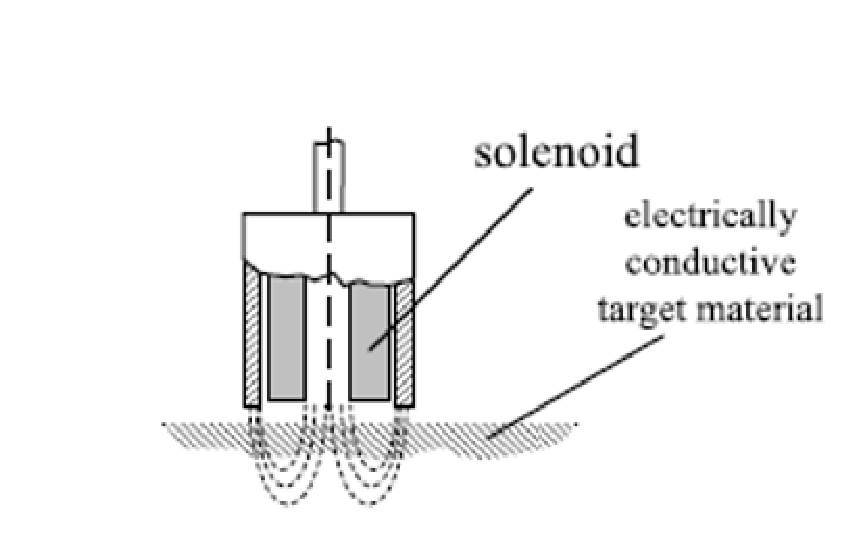
\includegraphics[width=5cm, height=4cm]{gap_sensor_1.eps}
	} 
	\subfigure[]{
		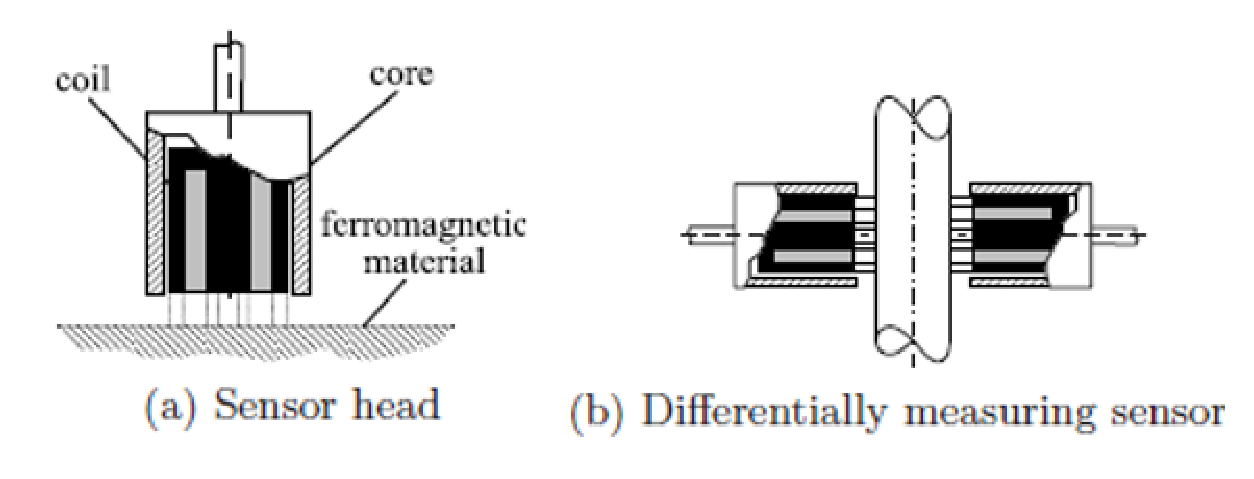
\includegraphics[width=8cm, height=4cm]{gap_sensor_2.eps}
	}
	\caption{Air gap measuring sensors (a) Eddy current displacement sensor, (b) Inductive displacement sensor.}
	\label{fig:gapsensor}
\end{figure}


\section{ABC} 
.......................
\subsection{SUB1-ABC}
.........................

\subsection{SUB2-ABC}
............................


% ---------------------------------------------------------------------------
%: ----------------------- end of thesis sub-document ------------------------
% ---------------------------------------------------------------------------
